\documentclass[10pt,aspectratio=169]{beamer}
\usepackage[T1]{fontenc}
\usepackage[utf8]{inputenc}
\usepackage{lmodern}
\usepackage{amsmath,amssymb}
\usepackage{booktabs,array}
\usepackage{graphicx}
\usepackage{tikz}
\usetikzlibrary{arrows.meta,positioning}
\graphicspath{{figures/}}

\usetheme{default}
\definecolor{navy}{RGB}{31,78,156}
\definecolor{brick}{RGB}{192,57,43}
\definecolor{leaf}{RGB}{46,139,87}
\definecolor{figorange}{RGB}{230,126,34}
\setbeamercolor{structure}{fg=navy}
\setbeamercolor{title}{fg=navy}
\setbeamercolor{frametitle}{fg=navy}
\setbeamercolor{block title}{bg=navy!12,fg=navy}
\setbeamercolor{block body}{bg=navy!4}
\setbeamercolor{alerted text}{fg=brick}
\setbeamertemplate{navigation symbols}{}
\setbeamertemplate{footline}{\hfill\scriptsize\color{black!55}\insertframenumber/\inserttotalframenumber\hspace{2ex}\vspace{1ex}}
\setbeamertemplate{itemize items}[circle]
\setbeamertemplate{caption}{\scriptsize\insertcaption}
\setbeamerfont{frametitle}{size=\large,series=\bfseries}
\setlength{\leftmargini}{1.2em}
\setlength{\emergencystretch}{2em}
\newcommand{\code}[1]{\texttt{\detokenize{#1}}}
\newcommand{\1}{\mathbf{1}}
\newcommand{\R}{\mathbb{R}}
\newcommand{\E}{\mathbb{E}}
\newcommand{\Reg}{\mathrm{Reg}}
\newcommand{\W}{\mathcal{W}}
\DeclareMathOperator*{\argmax}{arg\,max}
\DeclareMathOperator*{\argmin}{arg\,min}
\newcommand{\good}[1]{\textcolor{leaf}{#1}}
\newcommand{\bad}[1]{\textcolor{brick}{#1}}

\title{The SPO portfolio tree: model v1}
\subtitle{The model and its training, with the equations; then what the planted-threshold experiment says}
\author{Roman Beauvallet - Edo Theory}
\date{24 September 2026}



\begin{document}

\begin{frame}[plain]
\titlepage
\end{frame}

\begin{frame}{Outline}
\tableofcontents
\end{frame}

\section{What we do, and how we test it}
\begin{frame}{What we do, and how we test it}
\begin{columns}[T]
\column{0.5\textwidth}
\textbf{Problem}
\begin{itemize}
\item weights of $n$ assets every $h$ days, from features $x_t$, with fees
\item a decision problem, not a forecast
\end{itemize}
\medskip
\textbf{Model}
\begin{itemize}
\item small tree $\to$ leaf scores $\to$ mean--variance optimizer with fees
\item loss: decision regret through the optimizer
\item splits confirmed on the tree's own traded path
\item Out of sample Sharpe pruning 
\end{itemize}
\column{0.48\textwidth}
\textbf{Test}
\begin{itemize}
\item synthetic market, one feature $x$, planted threshold $d$
\item benchmark: \emph{ideal rule} = optimizer fed $\E[r\mid x]$
\item constant volatility; asset vs cash; weekly unless stated
\end{itemize}
\medskip
\textbf{Model v1}
\begin{itemize}
\item frozen 24 September 2026
\item $\approx15{,}000$ fitted trees behind the numbers
\item validated on 100 datasets
\end{itemize}
\end{columns}
\end{frame}

\section{The model: the tree, the decision problem, the loss, the training}
\begin{frame}{The tree: what a node stores}
\begin{columns}[T]
\column{0.57\textwidth}
\centering
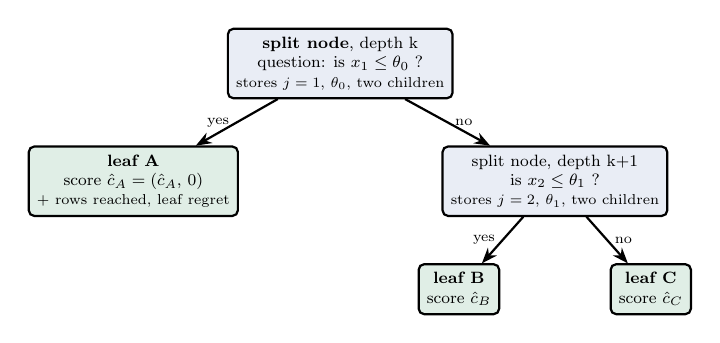
\begin{tikzpicture}[
  scale=0.74, every node/.style={transform shape, font=\footnotesize},
  split/.style={draw, thick, rounded corners=2pt, fill=navy!10, align=center, inner sep=4pt},
  leaf/.style={draw, thick, rounded corners=2pt, fill=leaf!15, align=center, inner sep=4pt},
  arr/.style={-{Stealth[length=2mm]}, thick}]
\node[split] (root) {\textbf{split node}, depth k\\ question: is $x_1\le\theta_0$ ?\\ {\scriptsize stores $j=1$, $\theta_0$, two children}};
\node[leaf, below left=0.8cm and -0.2cm of root] (A) {\textbf{leaf A}\\ score $\hat c_A=(\hat c_A,\,0)$\\ {\scriptsize + rows reached, leaf regret}};
\node[split, below right=0.8cm and -0.2cm of root] (S1) {split node, depth k+1\\ is $x_2\le\theta_1$ ?\\ {\scriptsize stores $j=2$, $\theta_1$, two children}};
\node[leaf, below left=0.8cm and -1.0cm of S1] (B) {\textbf{leaf B}\\ score $\hat c_B$};
\node[leaf, below right=0.8cm and -1.0cm of S1] (C) {\textbf{leaf C}\\ score $\hat c_C$};
\draw[arr] (root) -- node[left, font=\scriptsize] {yes} (A);
\draw[arr] (root) -- node[right, font=\scriptsize] {no} (S1);
\draw[arr] (S1) -- node[left, font=\scriptsize] {yes} (B);
\draw[arr] (S1) -- node[right, font=\scriptsize] {no} (C);
\end{tikzpicture}

\medskip
\medskip
\medskip
\medskip
\medskip
\medskip
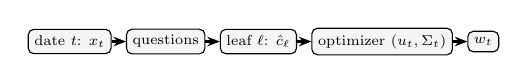
\begin{tikzpicture}[scale=0.74, every node/.style={transform shape, font=\scriptsize},
  box/.style={draw, rounded corners=2pt, inner sep=3pt, fill=black!4}, arr/.style={-{Stealth[length=1.6mm]}, thick}]
\node[box] (x) {date $t$: $x_t$};
\node[box, right=0.25cm of x] (route) {questions};
\node[box, right=0.25cm of route] (leaf) {leaf $\ell$: $\hat c_\ell$};
\node[box, right=0.25cm of leaf] (opt) {optimizer $(u_t,\Sigma_t)$};
\node[box, right=0.25cm of opt] (w) {$w_t$};
\draw[arr] (x) -- (route); \draw[arr] (route) -- (leaf); \draw[arr] (leaf) -- (opt); \draw[arr] (opt) -- (w);
\end{tikzpicture}
\column{0.41\textwidth}
\footnotesize
\begin{itemize}
\item tree = nested questions ``is $x_j\le\theta$?'', ending in leaves
\item \textbf{split node}: feature $j$, threshold $\theta$, two children; no score
\item \textbf{leaf}: one score vector $\hat c_\ell=(\hat c_\ell,\,0)$; rows reached; leaf regret
\item holdings $u_t$, weights $w_t$, returns: per date, not per node
\item depth $\le3$ $\Rightarrow$ $\le8$ leaves $\Rightarrow$ $\le8$ scores
\item growth: leaf $\to$ split node + 2 leaves; pruning: the reverse
\item use: $x_t\to$ leaf $\to\hat c_\ell\to$ optimizer$(u_t,\Sigma_t)\to w_t$
\end{itemize}
\end{columns}
\end{frame}

\begin{frame}{The decision: mean--variance with proportional fees}
\footnotesize
\begin{columns}[T]
\column{0.5\textwidth}
\textbf{Notation}
\begin{itemize}
\item $u$: holdings before the decision, $u_{t+1}=\dfrac{w_t\circ(1+r_t)}{1+r_t^\top w_t}$, $u_1=\1/n$
\item $c$: the tree's scores; cash $=0$ (cash earns nothing here + only the score differences matter)
\item $\Sigma$: $h$-day covariance from the last 180 days; $\sigma_h^2=h\hat\sigma^2$
\item $f$: 3 bp for the 11asset / 0 cash; $\lambda=1$
\item $\W=\{w:\,0\le w_i\le1,\ \sum_iw_i=1\}$
\end{itemize}
\column{0.48\textwidth}
\textbf{Properties}
\begin{itemize}
\item strictly concave $\Rightarrow$ unique $w^\star$
\item $w^\star(c+\alpha\1)=w^\star(c)$: only score differences matter
\item exact solution: 5 states per weight ($0$, cap$\ =\bar{w}$, $u_i$, buy, sell) $\Rightarrow$ $5^n$ linear systems, best feasible one
\end{itemize}
\end{columns}
\[
w^\star(c;u,\Sigma)=\argmax_{w\in\W}\ \underbrace{c^\top w}_{\text{gain}}-\underbrace{f^\top|w-u|}_{\text{fees}}-\underbrace{\lambda\,w^\top\Sigma w}_{\text{risk}}
\]
\textbf{Asset vs cash} ($w$ = asset weight, $\kappa=2\lambda\sigma_h^2$):
\[
w^\star=\begin{cases}
\min\{(c-f)/\kappa,\,1\} & c-\kappa u>f \ \text{(buy)}\\
\max\{(c+f)/\kappa,\,0\} & c-\kappa u<-f \ \text{(sell)}\\
u & |c-\kappa u|\le f \ \text{(no trade)}
\end{cases}
\]
\textbf{v1}: $\kappa=0.1\%$ (weekly, $\sigma=1\%$/day); $w:0\to1$ for $c:0.03\%\to0.13\%$/week; leaf scores $\pm0.3$--$0.5\%$ $\Rightarrow$ \alert{$w\in\{0,1\}$}; interior positions (continuous sizing)\ need $\lambda\ge5$
\end{frame}

\begin{frame}{The loss: decision regret; the score of a leaf}
\begin{align*}
U_t(w)&=r_t^\top w-f^\top|w-u_t|-\lambda\,w^\top\Sigma_t w\\
\Reg_t(c)&=U_t\big(w^\star(r_t;u_t,\Sigma_t)\big)-U_t\big(w^\star(c;u_t,\Sigma_t)\big)\ \ge0
\end{align*}
\centerline{\small hindsight decision $-$ decision on $c$ (given the same holdings $u_t$)}
\[
\hat c_\ell=\argmin_{c\in[-b,b]^n}\ \sum_{t\in\ell}\Reg_t(c),\qquad b=10\%
\]
\begin{columns}[T]
\column{0.48\textwidth}
\textbf{Leaf score}
\begin{itemize}
\item one regret per date, summed over the leaf's dates
\item bounded coordinate search: 3 passes $\times$ 7 values
\item not a forecast: same regret for any score on the right side
\end{itemize}
\column{0.48\textwidth}
\textbf{Consequences}
\begin{itemize}
\item fees $\Rightarrow$ regret depends on $u_t$ $\Rightarrow$ holdings from a replay of the tree
\item only differences: relative returns, asset vs cash $\implies$ help to choose the right features
\item same $\Sigma_t$ as the optimizer: unseen risk not learnt
\end{itemize}
\end{columns}
\end{frame}

\begin{frame}{Training: replay, two growth gates, out of sample pruning}
\begin{center}
\resizebox{0.9\textwidth}{!}{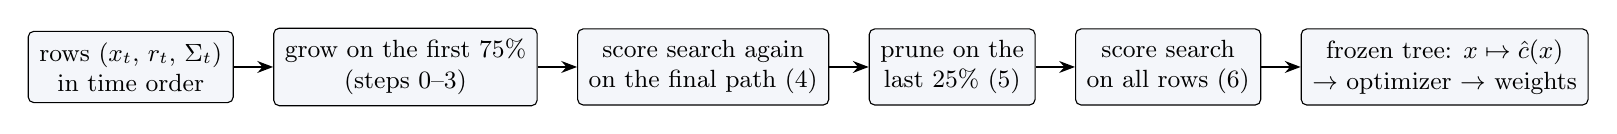
\begin{tikzpicture}[node distance=4mm and 5mm, every node/.style={font=\small},
  box/.style={draw, rounded corners=2pt, align=center, inner sep=4pt, fill=navy!5},
  arr/.style={-{Stealth[length=2mm]}, thick}]
\node[box] (rows) {rows $(x_t,\,r_t,\,\Sigma_t)$\\in time order};
\node[box, right=of rows] (grow) {grow on the first 75\%\\(steps 0--3)};
\node[box, right=of grow] (refit) {score search again\\on the final path (4)};
\node[box, right=of refit] (prune) {prune on the\\last 25\% (5)};
\node[box, right=of prune] (final) {score search\\on all rows (6)};
\node[box, right=of final] (use) {frozen tree: $x\mapsto\hat c(x)$\\$\to$ optimizer $\to$ weights};
\draw[arr] (rows) -- (grow); \draw[arr] (grow) -- (refit); \draw[arr] (refit) -- (prune); \draw[arr] (prune) -- (final); \draw[arr] (final) -- (use);
\end{tikzpicture}}
\end{center}
\footnotesize
\begin{enumerate}
\item[0.] root score from $u_t=\1/n$; \textbf{replay} (trade the scores date by date from $u_1$) $\Rightarrow$ $u_t$, hindsight utilities, Sharpe $S$; holdings frozen for the round
\item[1.] \textbf{regret gate}, per leaf: score search again from current $u_t$ (yardstick $L_\ell$); candidates; children of the 3 best; keep iff $\Delta=L_\ell-L_{\mathrm{left}}-L_{\mathrm{right}}>10^{-6}$ per row
\item[2.] \textbf{Sharpe gate}: rank all kept splits by $\Delta$; whole-tree replay of the first; accept iff $S'>S$, else next; one per round; none $\Rightarrow$ stop
\item[3.] replay the new tree $\Rightarrow$ new $u_t$; back to 1 (depth $\le3$; $\ge20$ rows and $\ge10\%$ of the parent per leaf)
\item[4.] score search again on every leaf, final path; kept iff $S$ does not fall
\item[5.] \textbf{pruning}, bottom-up, on the last 25\% (never used for growth): with vs without the split, both replayed;
$g_t=\Reg_t(\text{without})-\Reg_t(\text{with})$; keep iff $\bar g>10^{-6}$, $\ \bar g>k_p\,\mathrm{se}(\bar g)$ [$k_p=2$ below the root, $0$ at the root], checking Sharpe $\uparrow$
\item[6.] score search again on all training rows
\end{enumerate}
\textbf{Gates 1--2: in-sample. Gate 5: the only out-of-sample judge.}
\end{frame}

\section{Model v1: the split-search options and the frozen configuration}
\begin{frame}{Split-search options: quantile candidates, refinement, soft splits}
\scriptsize
\textbf{Common}: admissible candidates $\theta_{(1)}<\dots<\theta_{(K)}$ (each side $\ge m_\ast=\max(m,\lceil\varphi N\rceil)$ rows; $m=20$, $\varphi=10\%$); cheap screen
\[
Q(\theta)=\sum_{t\in I}\Reg_t\big(c_{\mathrm{side}(t)}(\theta)\big),\qquad c_{\mathrm{left}}(\theta)=\mathrm{clip}\big(\mathrm{mean}\{r_t: x_t\le\theta\},\pm b\big),\ \text{idem right}
\]
\begin{columns}[T]
\column{0.5\textwidth}
\textbf{Deciles by rank + refinement} 
\begin{itemize}
\item keep ranks $\mathrm{round}(q(K-1))$, $q=0.1,\dots,0.9$: 9 screens instead of $K\approx N-2m_\ast$
\item refinement: screen every candidate between the two deciles around the best one, $\theta_\circ$; best of them $\theta_\bullet$
\item replace iff $Q(\theta_\circ)-Q(\theta_\bullet)>k\,\mathrm{se}$, $\ \mathrm{se}=\sqrt{|I|}\,\mathrm{std}_t(\delta_t)$, $k=1$
\item 3 best survivors $\to$ full fit of the children
\end{itemize}
\column{0.48\textwidth}
\textbf{Soft split} (off in v1: $\kappa=0$)
\[
z_k=\frac{Q(\theta_k)-\min_lQ(\theta_l)}{\mathrm{se}_k},\qquad
\pi_k=\frac{e^{-z_k/\kappa}}{\sum_le^{-z_l/\kappa}}
\]
\begin{itemize}
\item all candidates kept, weighted; Gaussian variant $e^{-z^2/2\kappa^2}$
\item membership: left with $\mu(x)=\sum_{k:\,\theta_k\ge x}\pi_k$, right with $1-\mu(x)$; weights $\omega_{t\ell}$ multiply down the tree
\item leaf fit: $\min_c\sum_t\omega_{t\ell}\Reg_t(c)$; row score $\hat c(x_t)=\sum_\ell\omega_{t\ell}\hat c_\ell$: a ramp, not a jump
\item $\kappa\to0$: plain split
\end{itemize}
\end{columns}
\end{frame}

\begin{frame}{Model v1: the frozen configuration (24 September 2026)}
\scriptsize
\begin{tabular}{@{}p{2.4cm} p{4.6cm} p{6.4cm}@{}}
\toprule
Choice & v1 & Why (section of the experiments report) \\
\midrule
risk aversion $\lambda$ & 1 & positions 0/1: regime classifier, not sizer (8)\\
fee & 3 bp asset, 0 cash & market-sized; 10 bp starves fast rates (8)\\
decision rate & weekly ($h=5$); 2-day as alternative & daily $\approx$ weekly; monthly loses (4)\\
depth & $\le3$ & depth alone changes nothing (8)\\
leaf minimum & 20 decisions and 10\% of the node & tail leaves at 0.7\% of the data (7)\\
candidate thresholds & deciles by rank + refinement (1 s.e.) & = base Sharpe, steadier thresholds (9, 12)\\
soft splits & \textbf{off} & never raise the Sharpe at $\lambda=1$ (9, 12)\\
growth gates & regret reduction, then replayed Sharpe $\uparrow$ & kept as designed; v2 revisits\\
pruning & last 25\%; hurdle 2 s.e.\ below the root, none at the root & out-of-sample judge (7); removes spurious leaves at no cost (12)\\
covariance & 180-day window, $\Sigma_t=h\hat\sigma_t^2$ & 20-day window: noisier than timely (regime report)\\
conventions & cash column; all-cash Sharpe $=0$; $|\hat c|\le10\%$ & (7, model document)\\
\bottomrule
\end{tabular}

\medskip
\textbf{Base} of every experiment = same pipeline, every option off: depth 2, all candidates screened, plain pruning.
\end{frame}

\section{The planted-threshold experiment: recovery, performance, trading rate, what the options bought, v1 on 100 datasets, resolution}
\begin{frame}{The test-bed: a market with a planted answer (constant volatility)}
\begin{columns}[T]
\column{0.54\textwidth}
\small
\begin{gather*}
x_{t+1}=m+e^{-k}(x_t-m)+\eta_t,\quad \eta_t\sim\mathcal N\big(0,s^2(1-e^{-2k})\big)\\
\log\tfrac{S_{t+1}}{S_t}=\mu_t-\tfrac12\sigma^2+\sigma\varepsilon_t,\quad \mu_t=\pm e\sigma\ \text{as}\ x_t\gtrless d
\end{gather*}
\footnotesize
\begin{tabular}{@{}ll@{}}
\toprule
$\sigma$ & 1\% a day (16\%/yr), both regimes\\
$e$ (edge) & 0.10, 0.05, 0.02 $=\pm25$, $\pm13$, $\pm5\%$/yr\\
$k$ & 0.02/day (half-life 35 d); 0.01 to 0.10\\
$m, s^2, d$ & 0, 1, 0: threshold at the mean of $x$\\
$h$ & 1, 2, 5, 10, 21 days\\
data & 15 years training, 5 years test, daily\\
\bottomrule
\end{tabular}
\column{0.44\textwidth}
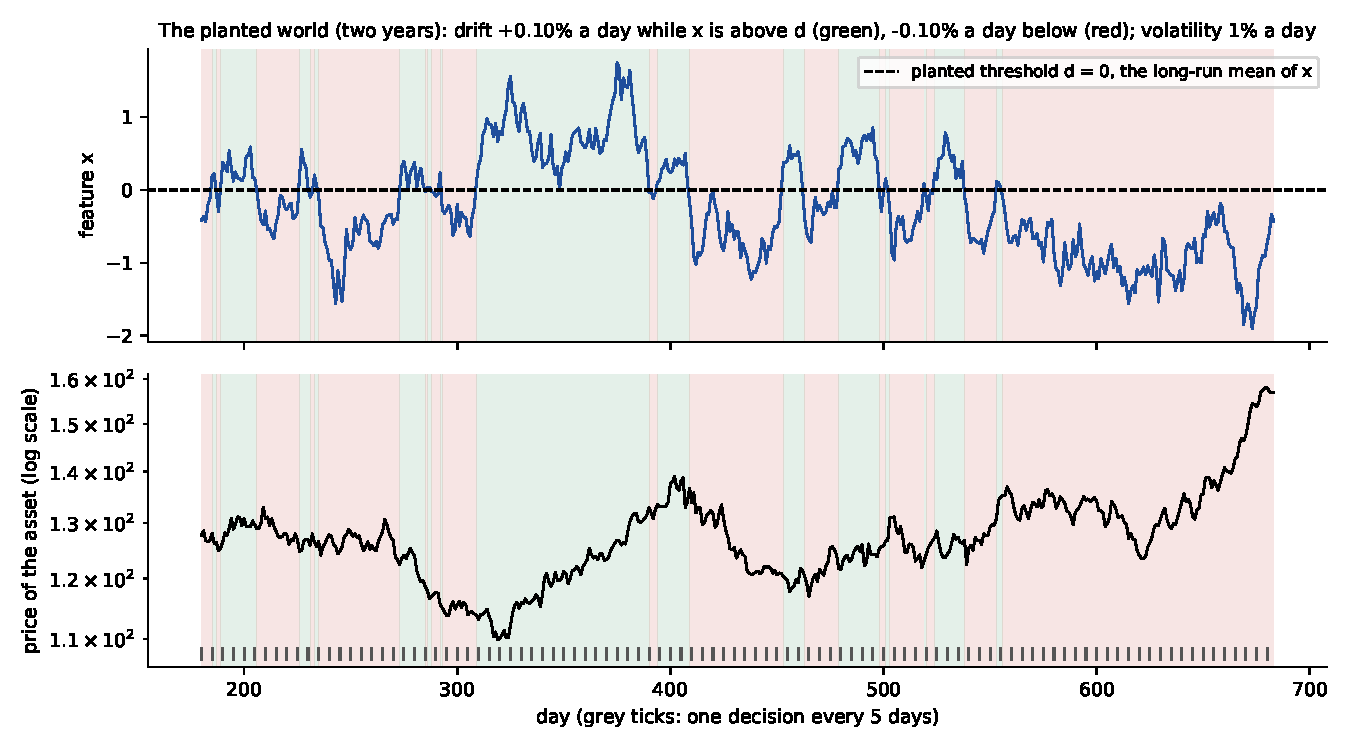
\includegraphics[width=\textwidth]{planted_world_one_dataset}
\footnotesize\textbf{Measured} (40--100 datasets per cell)
\begin{itemize}
\item first threshold vs planted $d=0$ ($x$ has sd 1)
\item annualized test Sharpe: tree vs ideal rule ($\E[r\mid x]$ fed to the optimizer), rule at $d$, always the asset
\item share of the ideal gain captured
\end{itemize}
Second market (volatility follows a threshold too): own report; one line at the end.
\end{columns}
\end{frame}

\begin{frame}{One fitted tree (dataset 42, weekly, edge 0.10)}
\begin{columns}[T]
\column{0.56\textwidth}
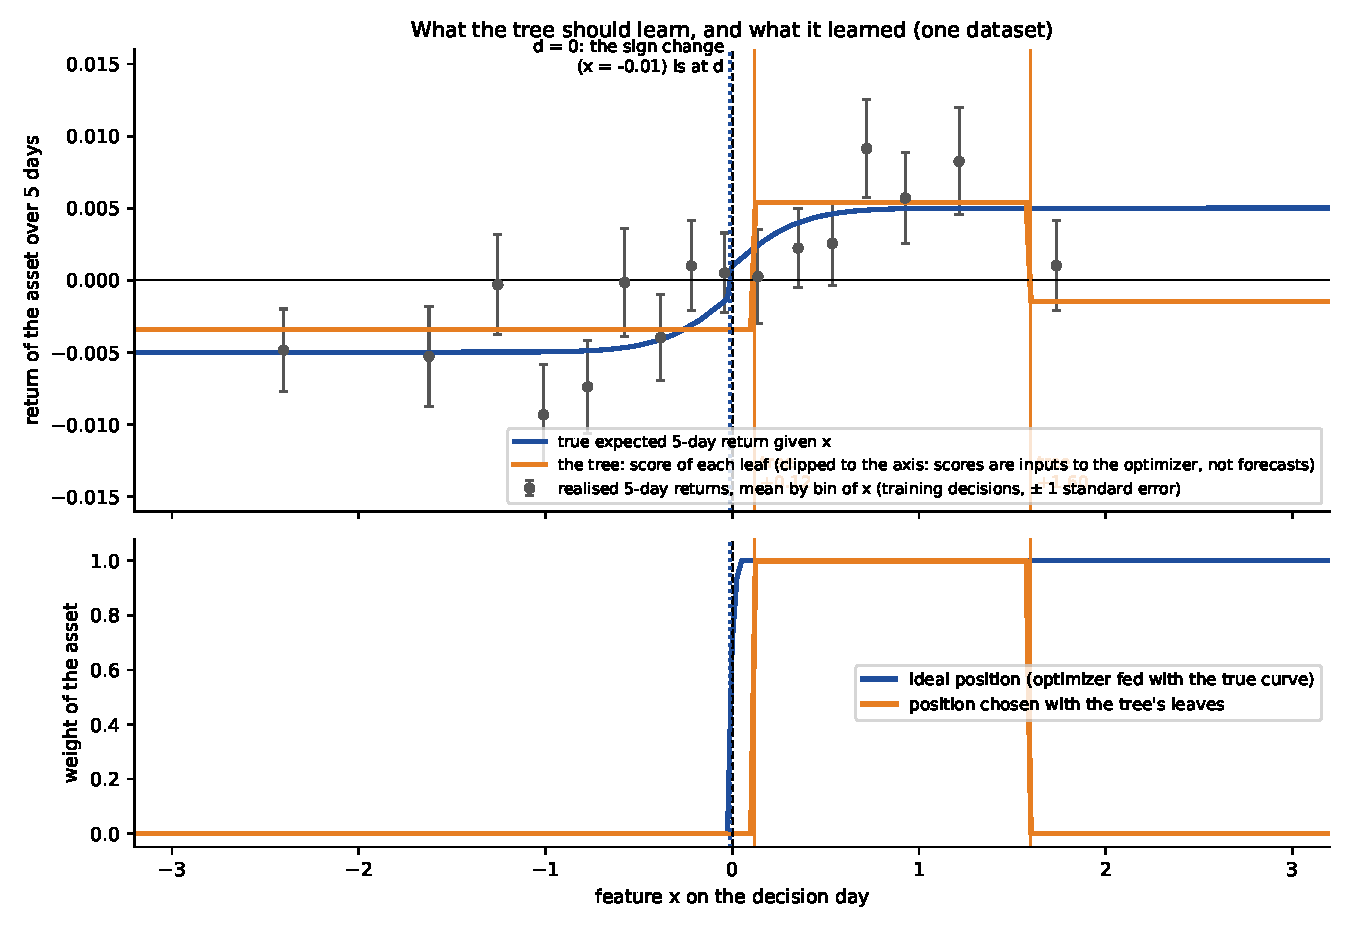
\includegraphics[width=\textwidth]{learned_vs_ideal_one_dataset}
\column{0.43\textwidth}
\scriptsize
\textbf{Drawn} ($x$ on the decision day)
\begin{itemize}
\item \textcolor{navy}{blue}: true $\E[r\mid x]$, 5-day; zero at $x=-0.01$
\item grey: realized 5-day returns, mean by bin of $x$, $\pm1$ s.e.
\item \textcolor{figorange}{orange}: the tree's score per leaf: $-0.35\%$ ($x\le0.12$), $+0.55\%$ (to $1.60$), $-0.15\%$ (above)
\item bottom: asset weight from a 50/50 portfolio, fed the curve (\textcolor{navy}{ideal}) or the score (\textcolor{figorange}{tree})
\end{itemize}
\textbf{Key points}
\begin{itemize}
\item root threshold $0.12$ vs planted $0$
\item scores $\ne$ curve, and need not be: both outside the $0.1\%$ window $\Rightarrow$ same positions as the ideal rule up to $1.60$
\item leaf above $1.60$: spurious (base pruning); cash where the ideal rule stays invested; removed by the v1 hurdle
\item ideal rule = a step too ($\lambda=1$)
\end{itemize}
\end{columns}
\end{frame}

\begin{frame}{Result 1: the threshold is recovered at market sizes (E2, base pipeline)}
\begin{columns}[T]
\column{0.5\textwidth}
\scriptsize\setlength{\tabcolsep}{3pt}
\begin{tabular}{@{}rr r c rr r@{}}
\toprule
& & split & threshold & \multicolumn{2}{c}{annual.\ test Sharpe} & \\
\cmidrule(lr){5-6}
edge & $h$ & on $x$ (\%) & within 0.25 & tree & ideal & gain\\
\midrule
0.10 & 1 & 97 & 95\% & 0.80 & 1.03 & 76\%\\
 & 5 & 94 & 81\% & 0.73 & 0.88 & 79\%\\
 & 21 & 81 & 60\% & 0.54 & 0.68 & 75\%\\
\addlinespace
0.05 & 1 & 82 & 60\% & 0.12 & 0.49 & 25\%\\
 & 5 & 78 & 53\% & 0.24 & 0.43 & 51\%\\
 & 21 & 62 & 34\% & 0.17 & 0.35 & 43\%\\
\addlinespace
0.02 & 5 & 54 & 26\% & $-0.03$ & 0.15 & $-3\%$\\
\bottomrule
\end{tabular}

\smallskip
\begin{itemize}
\item row = 100 datasets (50 at edge 0.02), threshold planted at $0$
\item split on $x$: trees keeping a split (else: no split at all)
\item within 0.25: first threshold within 0.25 sd of $x$ from $0$
\item Sharpe: mean over datasets, s.e.\ $\approx0.04$
\item gain: tree's excess test return over the no-split tree, as a share of the ideal rule's
\end{itemize}
\column{0.48\textwidth}
\small
\begin{itemize}
\item \textbf{$\pm25\%$/yr: found at every rate}; 95\% within 0.25 daily, 60\% monthly; 75--79\% of the ideal gain
\item \textbf{$\pm13\%$/yr: graceful degradation}; 62--82\% split; 25--51\% of a small gain (ideal 0.35--0.49)
\item \textbf{$\pm5\%$/yr: nothing to find in 15 years}; half no split, half at random; ideal rule $\approx0.15$; finding nothing = right answer
\item daily $\approx$ weekly; monthly loses (regime changes inside the holding period)
\end{itemize}
\end{columns}
\end{frame}

\begin{frame}{Result 2: the strategy's performance out of sample (E2, base pipeline)}
\begin{columns}[T]
\column{0.52\textwidth}
\scriptsize\setlength{\tabcolsep}{3pt}
\begin{tabular}{@{}rr rrrr r@{}}
\toprule
& & \multicolumn{4}{c}{annualized test Sharpe ratio} & gain\\
\cmidrule(lr){3-6}
edge & $h$ & tree & ideal rule & rule at $d$ & the asset & captured\\
\midrule
0.10 & 1 & 0.80 & 1.03 & 1.04 & $-0.02$ & 76\%\\
 & 2 & 0.86 & 0.97 & 0.98 & $-0.02$ & 85\%\\
 & 5 & 0.73 & 0.88 & 0.88 & $-0.02$ & 79\%\\
 & 10 & 0.63 & 0.78 & 0.78 & $-0.02$ & 78\%\\
 & 21 & 0.54 & 0.68 & 0.66 & $-0.02$ & 75\%\\
\addlinespace
0.05 & 1 & 0.12 & 0.49 & 0.49 & $-0.02$ & 25\%\\
 & 2 & 0.21 & 0.46 & 0.46 & $-0.02$ & 44\%\\
 & 5 & 0.24 & 0.43 & 0.42 & $-0.02$ & 51\%\\
 & 10 & 0.17 & 0.39 & 0.38 & $-0.02$ & 43\%\\
 & 21 & 0.17 & 0.35 & 0.34 & $-0.02$ & 43\%\\
\bottomrule
\end{tabular}

\smallskip
\begin{itemize}
\item 100 datasets per row; s.e.\ $\approx0.04$
\item ideal rule: optimizer fed $\E[r\mid x]$; rule at $d$: asset iff $x\ge d$; the asset: always invested
\item turnover per weekly decision (edge 0.10): tree 0.25, ideal 0.28 $\Rightarrow$ fees $\approx0.4\%$/yr
\end{itemize}
\column{0.46\textwidth}
\small
\begin{itemize}
\item \textbf{$\pm25\%$/yr: 75--85\% of the attainable gain} at every rate (0.73 vs 0.88 weekly; 0.86 vs 0.97 at 2 days)
\item \textbf{rule at $d$ = ideal rule}: at $\lambda=1$ the threshold is all there is to learn
\item lost: threshold error (0.07--0.25) + spurious leaves $\approx0.15$ Sharpe weekly
\item \textbf{$\pm13\%$/yr: 25--51\% of a small gain}: at the limit of what 15 years identify
\item always the asset: $\approx0$; the value is in the timing
\end{itemize}
\end{columns}
\end{frame}

\begin{frame}{Trading rate against the speed of the feature (edge 0.10, 50 datasets per cell)}
\begin{columns}[T]
\column{0.5\textwidth}
\scriptsize\setlength{\tabcolsep}{4pt}
\begin{tabular}{@{}l rr rr rr@{}}
\toprule
& \multicolumn{2}{c}{daily} & \multicolumn{2}{c}{weekly} & \multicolumn{2}{c}{monthly}\\
\cmidrule(lr){2-3}\cmidrule(lr){4-5}\cmidrule(lr){6-7}
half-life of $x$ & tree & ideal & tree & ideal & tree & ideal\\
\midrule
69 days ($k=0.01$) & 0.63 & 1.09 & 0.84 & 0.97 & 0.68 & 0.84\\
35 days ($k=0.02$) & 0.80 & 1.03 & 0.73 & 0.88 & 0.54 & 0.68\\
14 days ($k=0.05$) & 0.69 & 0.98 & 0.65 & 0.75 & 0.30 & 0.49\\
7 days ($k=0.10$) & 0.77 & 0.96 & 0.45 & 0.60 & 0.18 & 0.34\\
\bottomrule
\end{tabular}

\smallskip
annualized test Sharpe ratios, tree and ideal rule
\column{0.48\textwidth}
\small
\begin{itemize}
\item daily $\approx$ weekly: more decisions = more fees, not more information
\item monthly loses, more so for a fast feature: half-life 7 d $\Rightarrow$ 0.18 vs 0.34
\item slow feature + daily decisions: over-trading (0.63 vs 1.09)
\item $\Rightarrow$ weekly in v1
\end{itemize}
\end{columns}
\end{frame}

\begin{frame}{What the design options bought (E3--E5, E8; 40 datasets per cell, edge 0.10)}
\begin{columns}[T]
\column{0.46\textwidth}
\scriptsize\setlength{\tabcolsep}{2pt}
\begin{tabular}{@{}l cc@{}}
\toprule
& \multicolumn{2}{c}{test Sharpe of the tree}\\
\cmidrule(lr){2-3}
setting & weekly & 2-day\\
\midrule
base & 0.80 & 0.87\\
depth 3 & 0.80 & 0.89\\
$\lambda=5$ / $\lambda=10$ & 0.70 / 0.65 & 0.81 / 0.71\\
fee 10 bp & 0.60 & 0.53\\
deciles + refinement & 0.82 & 0.82\\
soft splits $\kappa=1$ & 0.53 & 0.35\\
soft splits $\kappa=0.25$ & 0.73 & 0.61\\
hurdle 2 s.e., every node & 0.43 & 0.47\\
hurdle 2 s.e., below the root only & 0.77 & 0.74\\
deciles + refin.\ + hurdle below root & 0.80 & 0.79\\
\bottomrule
\end{tabular}

\smallskip
base: depth 2, all candidates, plain pruning; ideal rule 0.91 weekly, 1.00 at 2 days; s.e.\ $\approx0.04$; last row = v1 at depth 2
\column{0.52\textwidth}
\footnotesize
\begin{itemize}
\item \textbf{no option beats the base beyond noise}; what is left is threshold noise
\item depth 3: nothing (a maximum); $\lambda=5$--$10$: gradual positions, learnt, $-0.1$ to $-0.15$; 10 bp: fast rates stop trading
\item deciles + refinement: = base, 9 candidates instead of hundreds, steadier thresholds $\Rightarrow$ \good{in v1}
\item soft splits: $\kappa=1$ score in the no-trade band; $\kappa=0.25$ = base from weekly on, loses at 2 days $\Rightarrow$ \bad{off} (smoothing the score $\ne$ sizing the position at $\lambda=1$)
\item hurdle at every node: loses true root splits (25\% block has no power at 2 s.e.) $\Rightarrow$ \bad{off}
\item hurdle below the root: second-level leaves 25/10/5/5\% $\to$ 5/0/0/0\%, no cost from weekly on $\Rightarrow$ \good{in v1}
\end{itemize}
\end{columns}
\end{frame}

\begin{frame}{Model v1 on 100 datasets (E9, 800 fits), paired with the base of Result 1}
\begin{columns}[T]
\column{0.58\textwidth}
\scriptsize\setlength{\tabcolsep}{3pt}
\begin{tabular}{@{}r r rr r r rr r@{}}
\toprule
& & \multicolumn{2}{c}{leaves} & 2nd level & within 0.25 & \multicolumn{2}{c}{Sharpe} & v1 $-$ base\\
\cmidrule(lr){3-4}\cmidrule(lr){7-8}
edge & $h$ & base & v1 & base $\to$ v1 & base $\to$ v1 & base & v1 & (2 s.e.)\\
\midrule
0.10 & 2 & 2.24 & 2.00 & 25 $\to$ 2\% & 92 $\to$ 89\% & 0.86 & 0.78 & $-0.08$ (0.07)\\
 & 5 & 2.14 & 1.94 & 18 $\to$ 0\% & 81 $\to$ 82\% & 0.73 & 0.73 & $+0.00$ (0.04)\\
 & 10 & 2.03 & 1.92 & 14 $\to$ 2\% & 70 $\to$ 72\% & 0.63 & 0.64 & $+0.01$ (0.05)\\
 & 21 & 1.90 & 1.81 & 9 $\to$ 0\% & 60 $\to$ 64\% & 0.54 & 0.53 & $-0.01$ (0.03)\\
\addlinespace
0.05 & 2 & 2.18 & 1.72 & 38 $\to$ 4\% & 64 $\to$ 57\% & 0.21 & 0.18 & $-0.03$ (0.06)\\
 & 5 & 2.01 & 1.80 & 21 $\to$ 3\% & 53 $\to$ 51\% & 0.24 & 0.22 & $-0.03$ (0.05)\\
 & 10 & 1.93 & 1.69 & 19 $\to$ 1\% & 47 $\to$ 49\% & 0.17 & 0.20 & $+0.03$ (0.04)\\
 & 21 & 1.76 & 1.59 & 13 $\to$ 0\% & 34 $\to$ 42\% & 0.17 & 0.14 & $-0.03$ (0.03)\\
\bottomrule
\end{tabular}

\smallskip
same 100 datasets (seeds 0--99); 2nd level: datasets keeping a second-level split; last column: mean paired difference of annualized test Sharpe, 2 s.e.\ in brackets; half of the datasets: identical Sharpe
\column{0.4\textwidth}
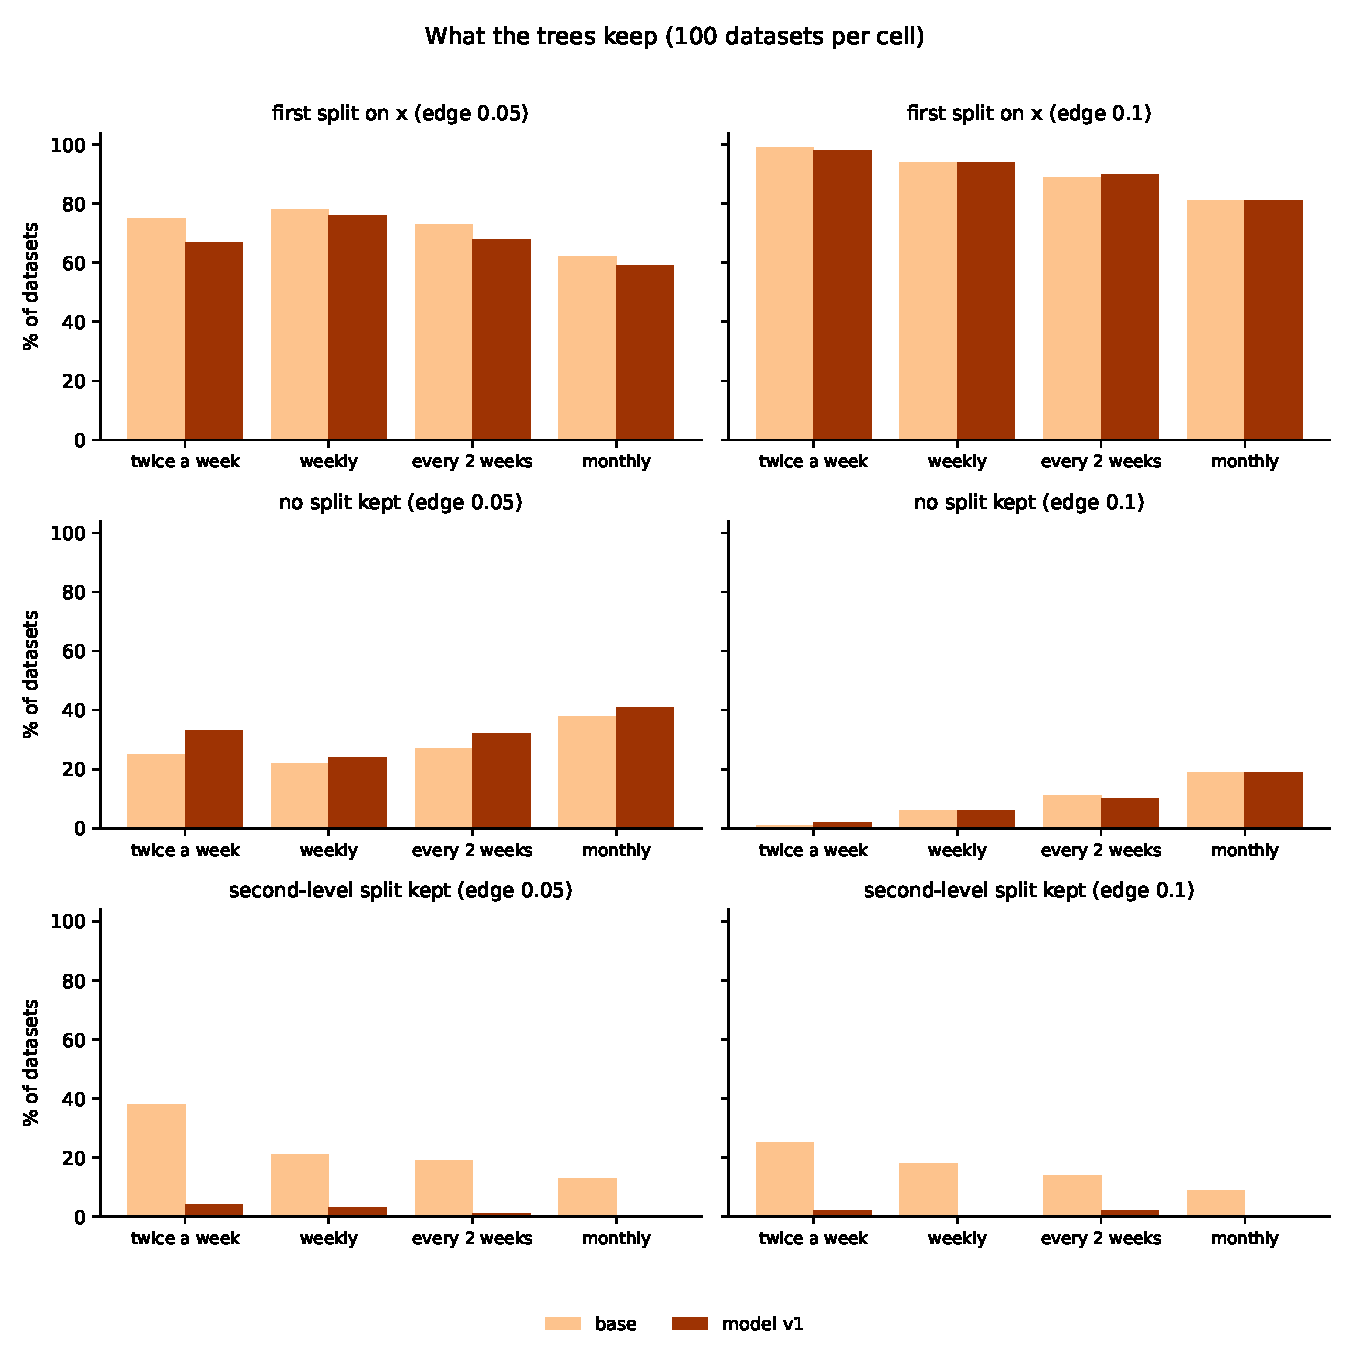
\includegraphics[width=0.78\textwidth]{model_v1_splits}
\scriptsize
\begin{itemize}
\item \good{weekly and slower: v1 = base within noise}; 2nd-level leaves gone; 1.9 leaves vs 2.1
\item \bad{2-day: $-0.08\pm0.07$ (edge 0.10)}: real 2nd-level splits removed; softer hurdle not run
\item depth budget unused ($\le1\%$ reach depth 2)
\item \textbf{v1 = base with a cleaner structure, not a higher Sharpe}
\end{itemize}
\end{columns}
\end{frame}

\begin{frame}{What can be found at all: resolution against volatility and feature noise (E6)}
\begin{columns}[T]
\column{0.52\textwidth}
\scriptsize\setlength{\tabcolsep}{3pt}
\begin{tabular}{@{}l l c c c@{}}
\toprule
sweep (weekly) & value & edge & median $|\theta|$ & tree / ideal\\
\midrule
volatility $\sigma$, drift $\pm25\%$/yr & 0.4\% & 0.25 & 0.05 & 1.85 / 2.10\\
 & 1.0\% & 0.10 & 0.12 & 0.69 / 0.87\\
 & 2.0\% & 0.05 & 0.39 & 0.23 / 0.42\\
 & 4.0\% & 0.025 & 0.95 & $-0.05$ / 0.18\\
\addlinespace
noise $\tau$ on $x$ & 0 & 0.10 & 0.12 & 0.69 / 0.87\\
 & 0.25 & 0.10 & 0.19 & 0.66 / 0.79\\
 & 0.5 & 0.10 & 0.25 & 0.45 / 0.66\\
 & 1 & 0.10 & 0.55 & 0.26 / 0.48\\
 & 2 & 0.10 & 1.15 & 0.09 / 0.29\\
\bottomrule
\end{tabular}

\smallskip
60 datasets per row; $|\theta|$: first threshold's distance from the planted $0$ (sd of $x$); $\tau$ in sd of $x$; tree / ideal: annualized test Sharpe
\column{0.46\textwidth}
\small
\begin{itemize}
\item threshold error $\approx0.012/e$ down to $e\approx0.05$; below: a guess
\item noise $\tau$ on $x$ $\approx$ edge divided by $1+\tau^2$
\item $\tau\le0.25$: free; $0.5$: error doubles; $1$: ideal Sharpe halves
\item edge below a few bp/day: unlearnable from 15 years, by any method
\item $\Rightarrow$ pre-test every real feature with this protocol
\end{itemize}
\end{columns}
\end{frame}

\section{A fair assessment, and what comes next}
\begin{frame}{A fair assessment, and what comes next}
\footnotesize
\begin{columns}[T]
\column{0.48\textwidth}
\begin{block}{Holds}
\begin{itemize}
\item $\pm25\%$ regime, monthly feature: recovered at every rate; 75--85\% of the attainable gain
\item $\pm13\%$: graceful; $\pm5\%$: correctly nothing
\item v1 = base with smaller trees, steadier thresholds (100 paired datasets); cost $0.08$ at 2 days
\item second market (volatility regime): drift threshold found better when the calm regime pays; a variance-only boundary not learnt (lagged covariance in the regret)
\end{itemize}
\end{block}
\column{0.5\textwidth}
\begin{block}{Weak or untested}
\begin{itemize}
\item no option beats the base beyond noise: structure, not Sharpe
\item growth Sharpe gate: in-sample, mixes a risk preference into the structure
\item one clean feature; synthetic data only; decoys only at an unrealistic edge; depth budget unused
\end{itemize}
\end{block}
\begin{block}{Next (v2)}
\begin{itemize}
\item growth gate off / replayed regret instead; same 100 datasets
\item regime-aware variance for optimizer and regret
\item two features + decoys at market-sized edges
\item real data; this protocol as the pre-test of every feature
\end{itemize}
\end{block}
\end{columns}
\end{frame}

\end{document}
